\documentclass[11pt]{article}
\usepackage{caption}
\usepackage{graphicx, subfig}
\title{The Computing Miniproject (Population Growth)}

\author{Dengkui Tang}

\date{Jan 2021}

\begin{document}
  \maketitle

  \begin{abstract}
    This paper will focus on the mathematical models of population growth (mechanistic) theory and phenomenological theory, by using different mathematical models to fit, to what extent do they fit the cross-species functional response data. This project is to use different models to show the growth curve of the whole microorganism. Then the model comparison methods is used to judge the advantages and disadvantages of these models. The fitting models are divided into two categories: linear models and nonlinear models. And this project mainly compares two nonlinear models, which are "logistic model" and "Gompertz model". The data used for the model fitting is called "LogisticGrowthData.csv", which are collected from laboratory experiments all around the world. After Python processes the data and then uses R to fit the models, the fitting curves corresponding to each "ID" are drawn. Finally, AIC and BIC are used to evaluate the models and get the conclusion. "Logistic model" is better than "Gompertz model" in this data set. 
  \end{abstract}

  \section{Introduction}
    Population growth rate is very important to biology. In a lot of biological research, researchers study a lot of specific questions and assumptions related to growth rates, such as the recently popular population growth rate, the growth rate of bacteria, the growth rate of microorganisms, and so on. All these studies need the support of logical evidence, mathematical modeling and computer knowledge. This study is a project of integrated population growth rate and computer mathematical modeling.

  \section{Methods}
    This project wants to show the population growth rate through graphs, and use different models to fit the growth rate data, and finally compare the advantages and disadvantages of different fitting models.
    \subsection{Computing tools}
    The programming tools used in this project are python and R language. In the Python script, it imports "Pandas", "Scipy", "csv" packages because the Python script is used to handle the data "ID". The R script is used for model fitting and drawing diagrams, so it requires "ggplot2" and "minpack.lm" packages. 
    \subsection{Data}
    There is a data set called LogisticGrowthData.csv, which contains measurements of biomass or microbial cell numbers over times. The data are collected from laboratory experiments all around the world. There is another data set called LogisticGrowthMetaData.csv that defined the field names for the above data set. The most two important set of data are "PopBio"(richness) and "Time". The growth rate curve of an individual population can be identified by a unique temperature-species-medium-citation-replicate combination. 
        \subsubsection{Data processing}
        "PopBio" and "Time" sets can be used directly. The "ID", however, need to be handled separately. The "ID" should contain "Species", "Medium", "Temp", and "Citation". In this case, "data.insert()" is used in a python script in order to combine these four columns into a new column called "ID". The processed data is than stored in a new CSV file called GrowthData.csv. 
    \subsection{OLS}
    OLS regression is the prediction of quantified dependent variables by the weighted sum of the predictive variables, where the weights are the parameters obtained by data estimation. In R, the most basic function for fitting a linear model is lm ():
    \begin{equation}
        lm\_growth <- lm(log(PopBio)\wr Time,current\_df)
    \end{equation}
    \subsection{NLLS}
    For nonlinear fitting model, this project selects two classical algorithms, which are "Logistic model" and "Gompertz model". Then these two models' functions are needed to fit the data. Here are the equations for the two models:
        \subsubsection{Logistic model}
        \begin{equation}
            N_{t}=\frac{N_{0} Ke^{rt}}{K+N_{0}(e^{rt}-1)} 
        \end{equation}
        For this model, there are three initial parameters that need to be defined separately: N\_0\_start should be the minimize "PopBio", N\_max\_start should be the maximize "PopBio", r\_max\_start should be the slope of growth rate (which can be calculated from OLS). 
        \subsubsection{Gompertz model}
        \begin{equation}
            \log (N_{t})=N_{0} + (N_{max}-N_{0})e^{-e^{rmax\exp (1)\frac{t_{lag^{-t}}}{(N_{max}-N_{0})\log (10)}+1}}
        \end{equation}
        For this model, there are four initial parameters that need to be defined separately: N\_0\_start should be the minimize "PopBio", K\_start should be the maximize "PopBio", r\_max\_start should be the slope of growth rate (which can be calculated from OLS), t\_lag\_start should be the last timepoint of lag phase.
        \subsubsection{Graphs}
        Different ID data need to be processed separately, so a large loop is used to separate the data of each group of ID for model fitting. According to the above two model equations, the fitting results are plotted by ggplot method.
        \begin{figure}
          \centering
          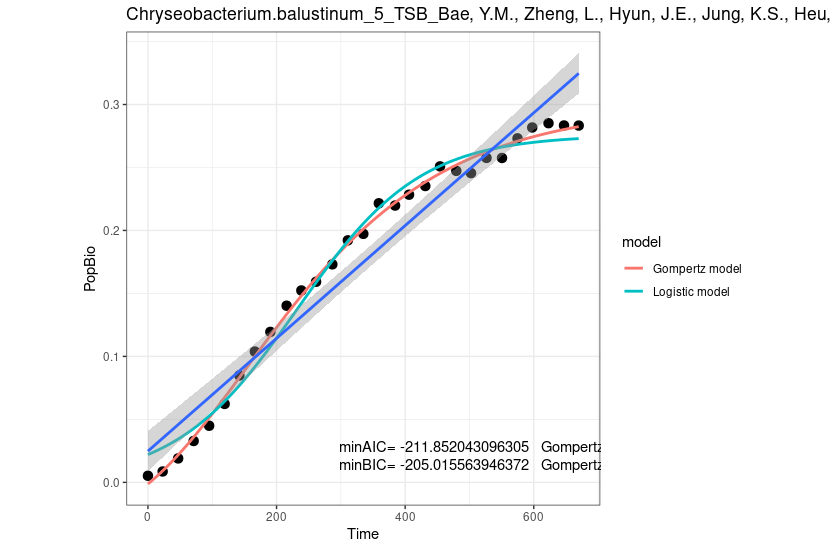
\includegraphics[width=.8\textwidth]{../results/Rplot.png}
        \end{figure}
        
  \section{Results}
    Often, when modeling a bunch of data, especially classification and regression models, there are many variables available. And choosing different combinations of variables can result in different models.
    There are the parameters for the following two models: L is the maximum likelihood under the model, N is the number of data, and K is the number of variables in the model.
	\subsection{AIC}
	\begin{equation}
    	AIC = 2k - 2 \ln(L)
  	\end{equation}
    The Akaike Information Criterion, which called "AIC", is a standard to measure the fitness of statistical models. It was created and developed by Japanese statistician Hiroji Akaike. Akakike information criterion is based on the concept of entropy. Increasing the number of free parameters improves the goodness of fitting. AIC encourages the goodness of data fitting but tries to avoid the situation of over-fitting. Therefore, the preferred model should be the one with the smallest AIC value. Assuming that the choice is made among n models, the AIC value of n models can be calculated at one time, and the model corresponding to the minimum AIC value can be found as the selection object. Generally, when the model complexity increases (k), the likelihood function L will also increase, thus reducing AIC. However, when k is too large, the likelihood function will increase slowly, which leading to the increase of AIC. Overfitting phenomenon may easily occur when the model is too complex. The smaller the AIC, the better the model, and the model with the smallest AIC is usually chosen.
	\subsection{BIC}
    \begin{equation}
    	BIC = \ln(n)k - 2\ln(L) 
  	\end{equation}
    The penalty term of BIC is larger than that of AIC, taking into account the number of samples. When the number of samples is too large, it can effectively prevent the model complexity caused by the high accuracy of the model. The principles of AIC and BIC are different. AIC selects a good model for prediction from the perspective of prediction, while BIC selects a model that best fits the existing data from the perspective of fitting. In terms of the interpretation of Bayesian factor, it is the model with the largest marginal likelihood
    \subsection{Model fitting result}
    The processed data table "GrowthData.csv" has 285 different "IDs" in total. Model fitting was carried out with OLS and NLLS for the data under each different "IDs", and charts were drawn. AIC and BIC were used to analyze and judge the fitting results of these 285 groups. The results were as follows: When AIC was used for judgment, the AIC calculation result of "Logistic Model" was 207 times less than that of "Gompertz Model", while the AIC calculation result of "Gompertz Model" was 78 times less than that of "Logistic Model". Therefore, according to AIC judgment, "Logistic Model" is superior to "Gompertz Model". When BIC was used for judgment, the BIC calculation result of "Logistic Model" was 211 times less than that of "Gompertz Model", while the BIC calculation result of "Gompertz Model" was 74 times less than that of "Logistic Model". Therefore, according to BIC judgment, "Logistic Model" is superior to "Gompertz Model". In conclusion, for the data set given, "Logistic Model" is better than "Gompertz Model" in both AIC and BIC judgments. 
  \section{Discussion}
    At the end of the paper, the goal of this project is to analyze the growth rate data and present it through model fitting, and to judge whether the model fitting is good or bad through model fitting criteria. To sum up, this project is basically realized. The main finding is that the "logistics model" is more relevant to the population growth rate data than the "Gompertz model". 
  
\end{document}
